\chapter{Empirical Study and Analysis}
We provide more empirical study results on the \texttt{MultiAgencyNews} dataset by comparing news articles from left- and right-wing news agencies. We present a word cloud visualization of the news article contents in \refsec{empirical-wordcloud}, a topic modeling visualization with LDA in \refsec{empirical-lda}, an AMR graph visualization in \refsec{empirical-amr}, and a PVI baseline with a BERT backbone in \refsec{empirical-bert-pvi}. 

For the word cloud, LDA visualization, and AMR visualization, the topic of their corpus is gun control\footnote{\url{https://ground.news/interest/gun-control}}. For the BERT PVI baseline, the whole dataset is used.

\section{Word Cloud by Frequency}
\label{empirical-wordcloud}
The news article content of a gun control news\footnote{\url{https://tinyurl.com/2nzw6c3m}} is modeled with word cloud\footnote{\url{https://pypi.org/project/wordcloud/}} and shown in \reffig{fig:empirical-wordcloud-left}. On the Left side, the discussion is inclined towards the assault weapons themselves and their consequences, while on the Right side discussion is inclined towards the bill itself, the opponents' partisanship, and political concepts.

\begin{figure}[ht]
    \centering
    \begin{minipage}[b]{0.45\textwidth}
        \captionsetup{justification=centering}
        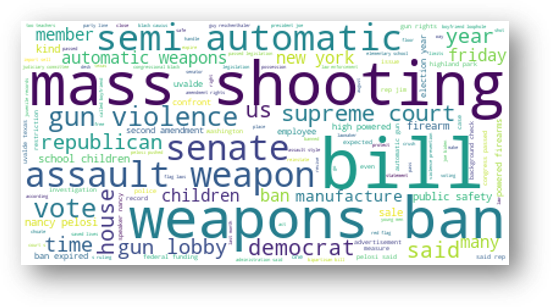
\includegraphics[width=\textwidth]{img/empirical-wordcloud-left}
        \caption{Wordcloud of Left-wing News Articles.}
        \label{fig:empirical-wordcloud-left}
    \end{minipage}
    \hfill
    \begin{minipage}[b]{0.45\textwidth}
        \captionsetup{justification=centering}
        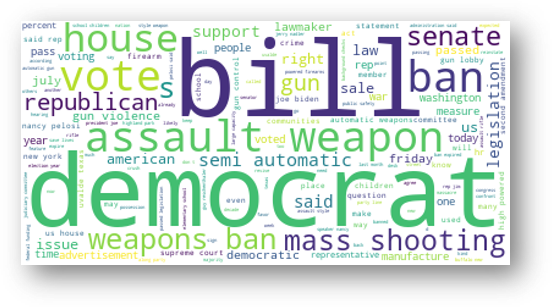
\includegraphics[width=\textwidth]{img/empirical-wordcloud-right}
        \caption{Wordcloud of Right-wing News Articles.}
        \label{fig:empirical-wordcloud-right}
    \end{minipage}
\end{figure}

\section{Topic Modeling with LDA}
\label{empirical-lda}
We also apply Latent Dirichlet Allocation (LDA) topic modeling on the dataset to compare the topics on both sides. The results are shown in \reffig{fig:empirical-lda-left} and \reffig{fig:empirical-lda-right}. On the Left side, topics are more dispersed, and the discussion on the ban itself is equivalent to weapons, while on the Right side topics are more focused, and the largest topic emphasizes the ban itself more than the weapons.

\begin{figure}[ht]
    \centering
    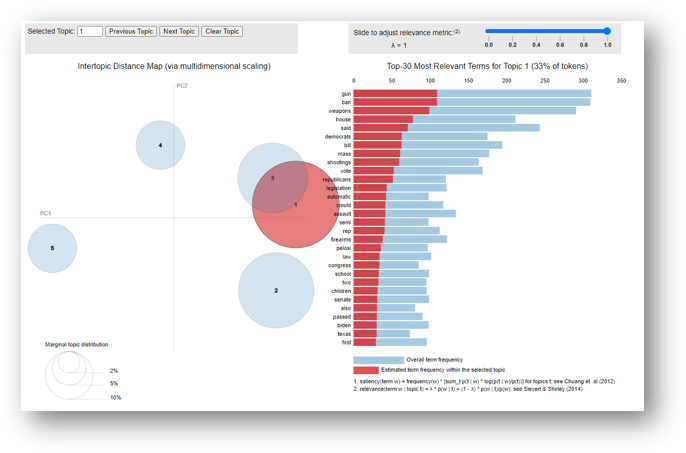
\includegraphics[width=0.8\textwidth]{img/empirical-lda-left}
    \caption{LDA Topic Modelling Result of Left-wing News Articles.}
    \label{fig:empirical-lda-left}
\end{figure}
\begin{figure}[ht]
    \centering
    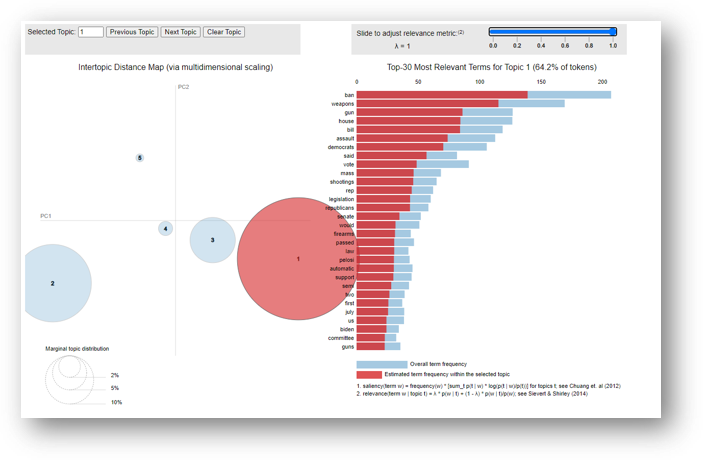
\includegraphics[width=0.8\textwidth]{img/empirical-lda-right}
    \caption{LDA Topic Modelling Result of Right-wing News Articles.}
    \label{fig:empirical-lda-right}
\end{figure}

\section{AMR Graph Modeling}
\label{empirical-amr}
The Abstract Meaning Representation (AMR) graphs are also extracted to compare the article structures on both sides. The results are shown in \reffig{fig:empirical-amr-left} and \reffig{fig:empirical-amr-right}. In addition to the basic facts (shooter age, place of incident, \etc), the news article on the Left side pointed out the emotions (``sad'' / ``anger''), while the news article on the Right side emphasizes the critical injury to the officer (``situation'' / ``critical'').

\begin{figure}[ht]
    \centering
    \captionsetup{justification=centering}
    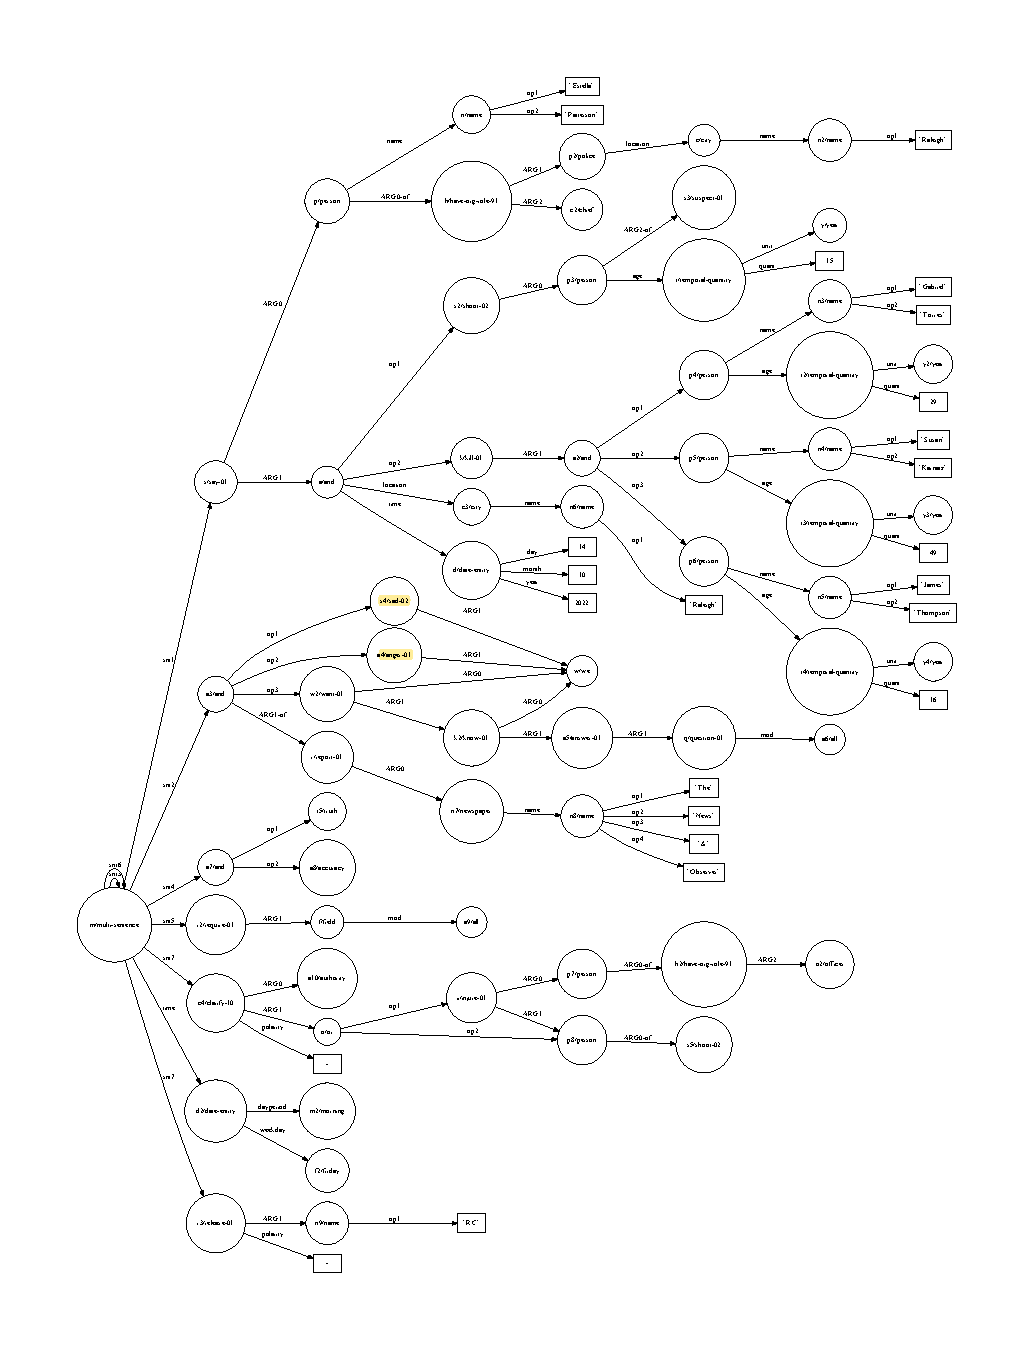
\includegraphics[width=0.9\textwidth]{img/empirical-amr-left}
    \caption{The AMR Graph of Left-wing News Articles.}
    \label{fig:empirical-amr-left}
\end{figure}
\begin{figure}[ht]
    \centering
    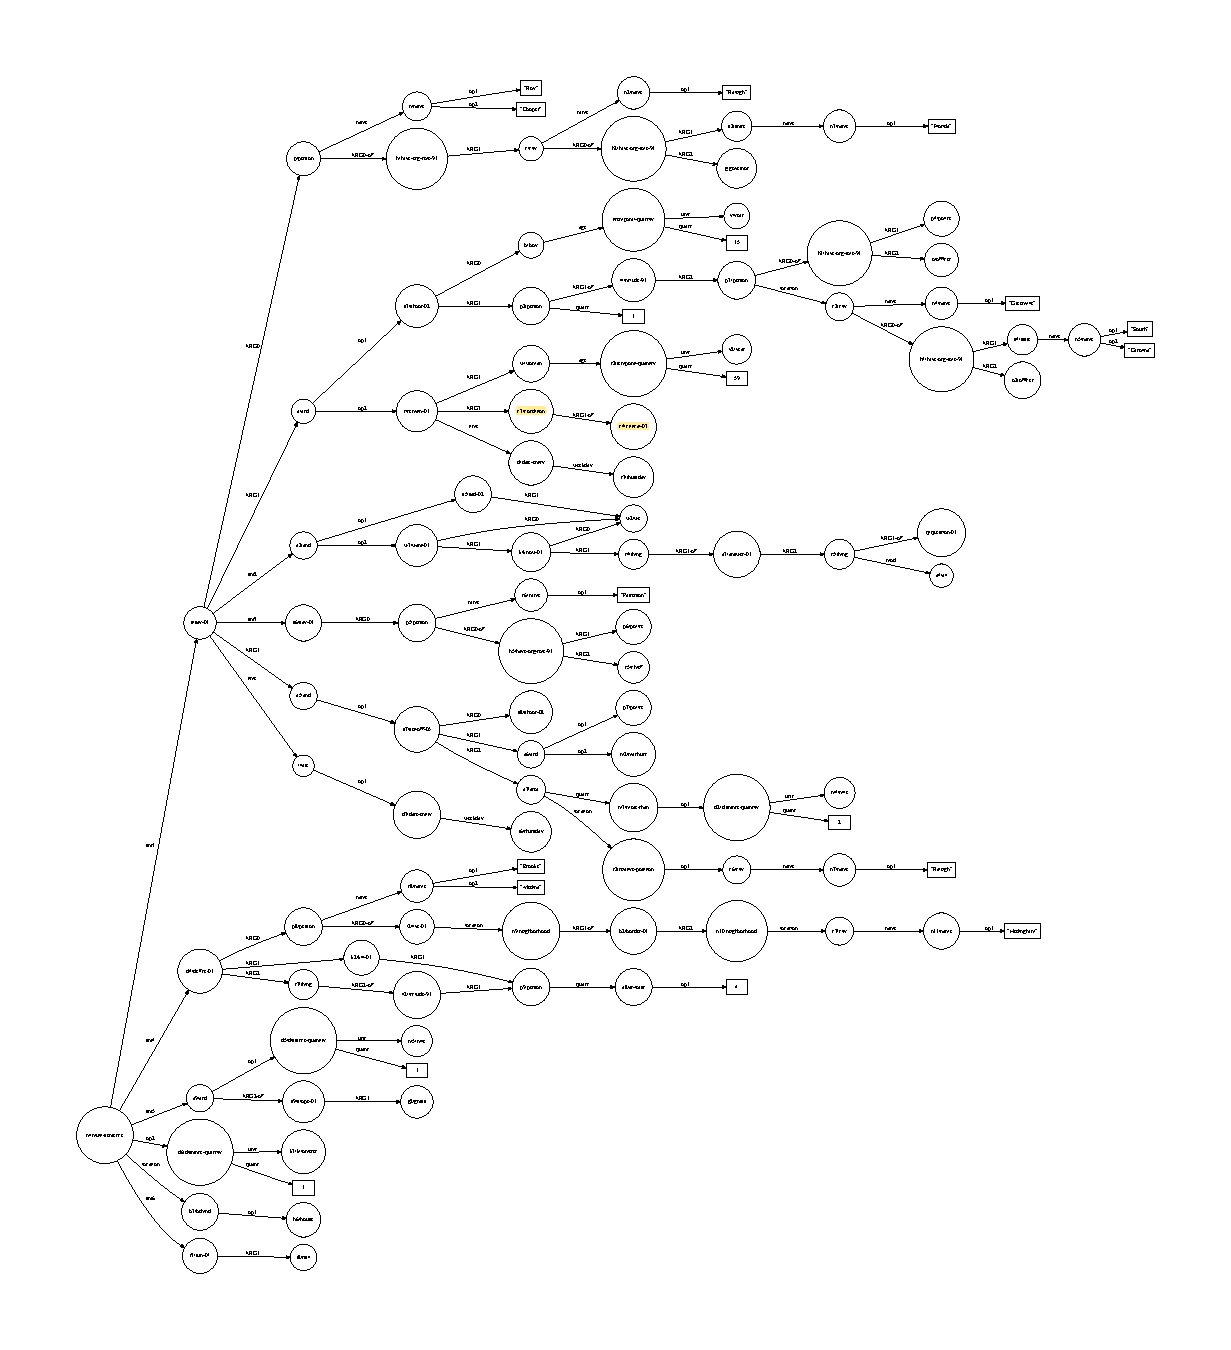
\includegraphics[width=\textwidth]{img/empirical-amr-right}
    \caption{The AMR Graph of Right-wing News Articles.}
    \label{fig:empirical-amr-right}
\end{figure}
\clearpage

\section{BERT PVI Baseline}
\label{empirical-bert-pvi}
To evaluate how challenging the dataset is for Political Viewpoint Identification (PVI), we finetuned a BERT model for sequence classification. The finetuning started with a vanilla bert-base-uncased checkpoint from HuggingFace Transformers\footnote{\url{https://huggingface.co/bert-base-uncased}}. The task is formulated as a 2-way classification with binary cross entropy loss. The dataset was split into training, validation, and test sets at the ratio of 0.7/0.1/0.2. The results are shown in \reffig{fig:empirical-bert-baseline}. The baseline model achieved only 59.19\% accuracy on the test set, which is only marginally higher than random guessing. This implies that PVI on the \texttt{MultiAgencyNews} dataset is still a challenging task.

\begin{figure}[ht]
    \centering
    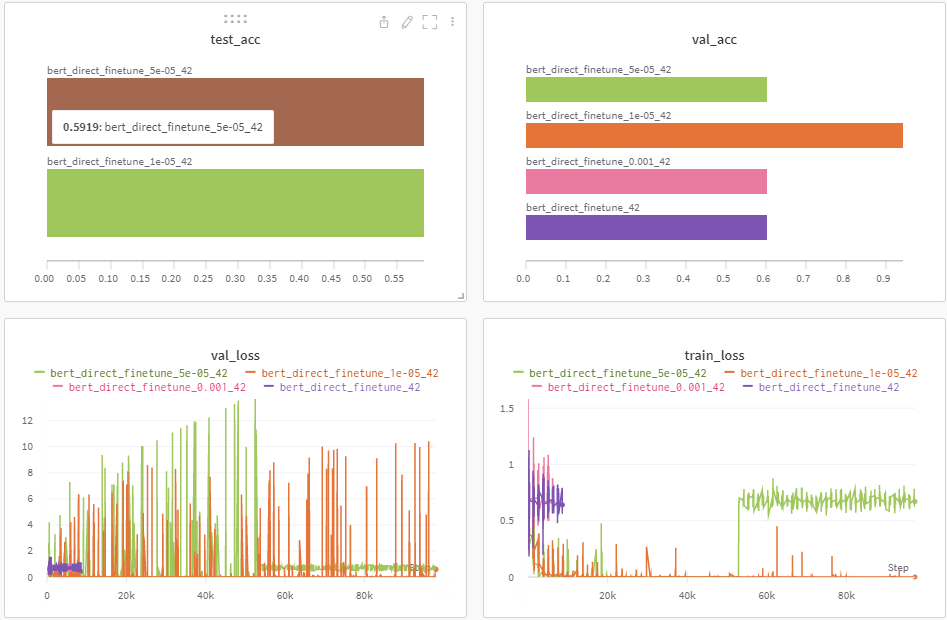
\includegraphics[width=\textwidth]{img/empirical-bert-baseline}
    \caption{The AMR Graph of Left-wing News Articles.}
    \label{fig:empirical-bert-baseline}
\end{figure}
